\section{Rooms-based Symmetry Reduction}
\begin{figure}[]
       \begin{center}
                       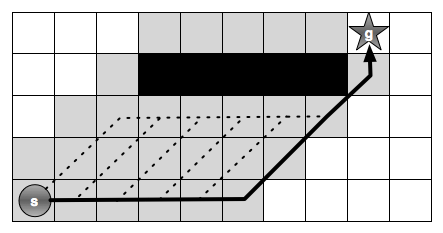
\includegraphics[scale=0.40]{diagrams/symmetry_example.png}
       \end{center}
       \caption{A pathfinding instance with high symmetry. We highlight the
eventual solution returned by A* (strong line) and a number of symmetric 
alternatives (dashed lines).}
       \label{fig-symmetry}
		\vspace{-0.5em}
\end{figure}
Symmetry is generally regarded as an undesirable characteristic in a search
space.
In the presence of symmetry, search algorithms are usually forced to evaluate 
many equivalent states, wasting time and making little real progress toward the goal.
Consider for example Figure \ref{fig-symmetry} where the majority of search
effort is expended evaluating nodes on symmetric paths to the eventual solution.
\par
The problem of how to deal with symmetry is well studied and appears regularly
in the literature; usually in the context of planning and constraint programming
but also bin packing and operations research. 
Despite this, there are very few works that explicitly identify and deal with the 
problem of symmetry in a pathfinding context. To address this, we begin by first
making precise the notion of symmetric relationship between paths:
\begin{definition}
Two paths $\pi_{1}$ and $\pi_{2}$ are symmetric if they share the same start and
goal node and one can be derived from the other by interchanging the order of the
moves.
\end{definition}

We will employ the following high-level strategy to
identify and eliminate path symmetries from 4 and 8-connected uniform cost grid maps:
\input alg_rsr

In \cite{harabor10} the same approach is used to develop the 4ERR algorithm.
Here, we extend that work as follows:
\begin{enumerate}
\item{
We extend Step \ref{alg:rsr:2} of Algorithm \ref{alg:rsr} 
to include pruning of nodes from the perimeter of an empty room.
}
\item{
We modify Steps \ref{alg:rsr:3} and \ref{alg:rsr:4} of Algorithm
\ref{alg:rsr} in order to facilitate optimal room traversal in 8-connected grid
maps. 
\item{We introduce a new online pruning strategy that allows faster node
expansion and further speeds up search.}
}
\end{enumerate}
As we will see, the first enhancement can significantly reduce the number of nodes
in the search space and results in a considerable speedup when compared to 4ERR.
The generalisation to 8-connected grids however is more challenging.
In particular, the branching factor associated with each remaining perimeter tile 
can become linear in the size of the largest dimension (length or width) of the local room. 
This number is often much larger than 8. 
By comparison, on a 4-connected map no tile requires more than one macro-edge 
to retain optimality and thus the branching factor remains low.
Keeping the branching factor within reasonable limits on 8-connected maps
is the primary motivation
for our final enhancement: a novel online pruning strategy which attempts to
reduce the number of neighbours that need to be considered during each node 
expansion operation.
%\par
%Both speedup enhancements, which we discuss in an upcoming section,
%are applicable to 4 and 8-connected grid maps and both preserve optimality
%during search.
%We term the resultant algorithm \emph{Rooms-based Symmetry Reduction} 
%(or RSR for short).
%\newline \\
%\textbf{Symmetry Reduction in 8-connected Grid Maps:}
%Consider a path which enters an empty room $R$ at some perimeter node $m$ and exits at some other
%node $n$ located on the opposite side of the room.
%On a 4-connected map we can optimally traverse the room by expanding $m$, following
%its macro edge to a node $m'$ on the opposite side of $R$ and finally navigating from $m'$ to $n$.
%The length of this path is equal to the Manhattan distance between $m$ and $n$ and thus optimal.
%However, if the map consists of 8-connected tiles this strategy is no longer optimal.
%In particular, the original (unmodified) map may contain a more direct path to $n$ using one or more diagonal
%transtions.
%\par
%We address this problem as follows:
%First, we give an offline procedure which adds to $R$ a set of additional macro edges
%to facilitate optimal travel between arbitrary pairs of tiles on the perimeter.
%Second, we give an online re-insertion procedure which deals with cases where the start or
%goal is a tile that has been previously removed.
%Finally, we show that this method preserves optimality.
